\subsubsection{概要}
しらたまチームは1章で述べた目標のために, 
上田研究室に保存されているドキュメントを用いてロボットのセットアップや実装を行った. 
しらたまチームでは, 自己位置推定にemcl2\_ros2,ナビゲーションにnavigation2を採用した. 

%開発してないので省略
%\subsubsection{開発したパッケージ}

%システム図作成する必要あり
\subsubsection{システム構成}
ロボットに搭載した計算機,センサ,
アクチュエータの接続の関係及び計算機で実行するROS 2ノードの概要を表したものを図\ref{fig:shiratama_system}に示す. 

Raspberry Piには, 車体制御のために, エンコーダと車輪駆動用のモータを接続した. 
実行するノードとしては, 

\begin{itemize} 
\item urg\_node: レーザにより周囲の障害物との距離を測定し,スキャンデータとして配信. 

\item raspimouse: ロボットの駆動制御を行う.また,エンコーダの代わりに,速度指令値(cmd\_vel)をオドメトリの情報(/odom)として配信する.

\item map\_server: 事前に作成した環境地図を配信.

\item emcl2: モンテカルロ自己位置推定(MCL)を実行するノード.
\end{itemize}
%something
がある.  


\begin{figure}[h]
  \begin{center}
    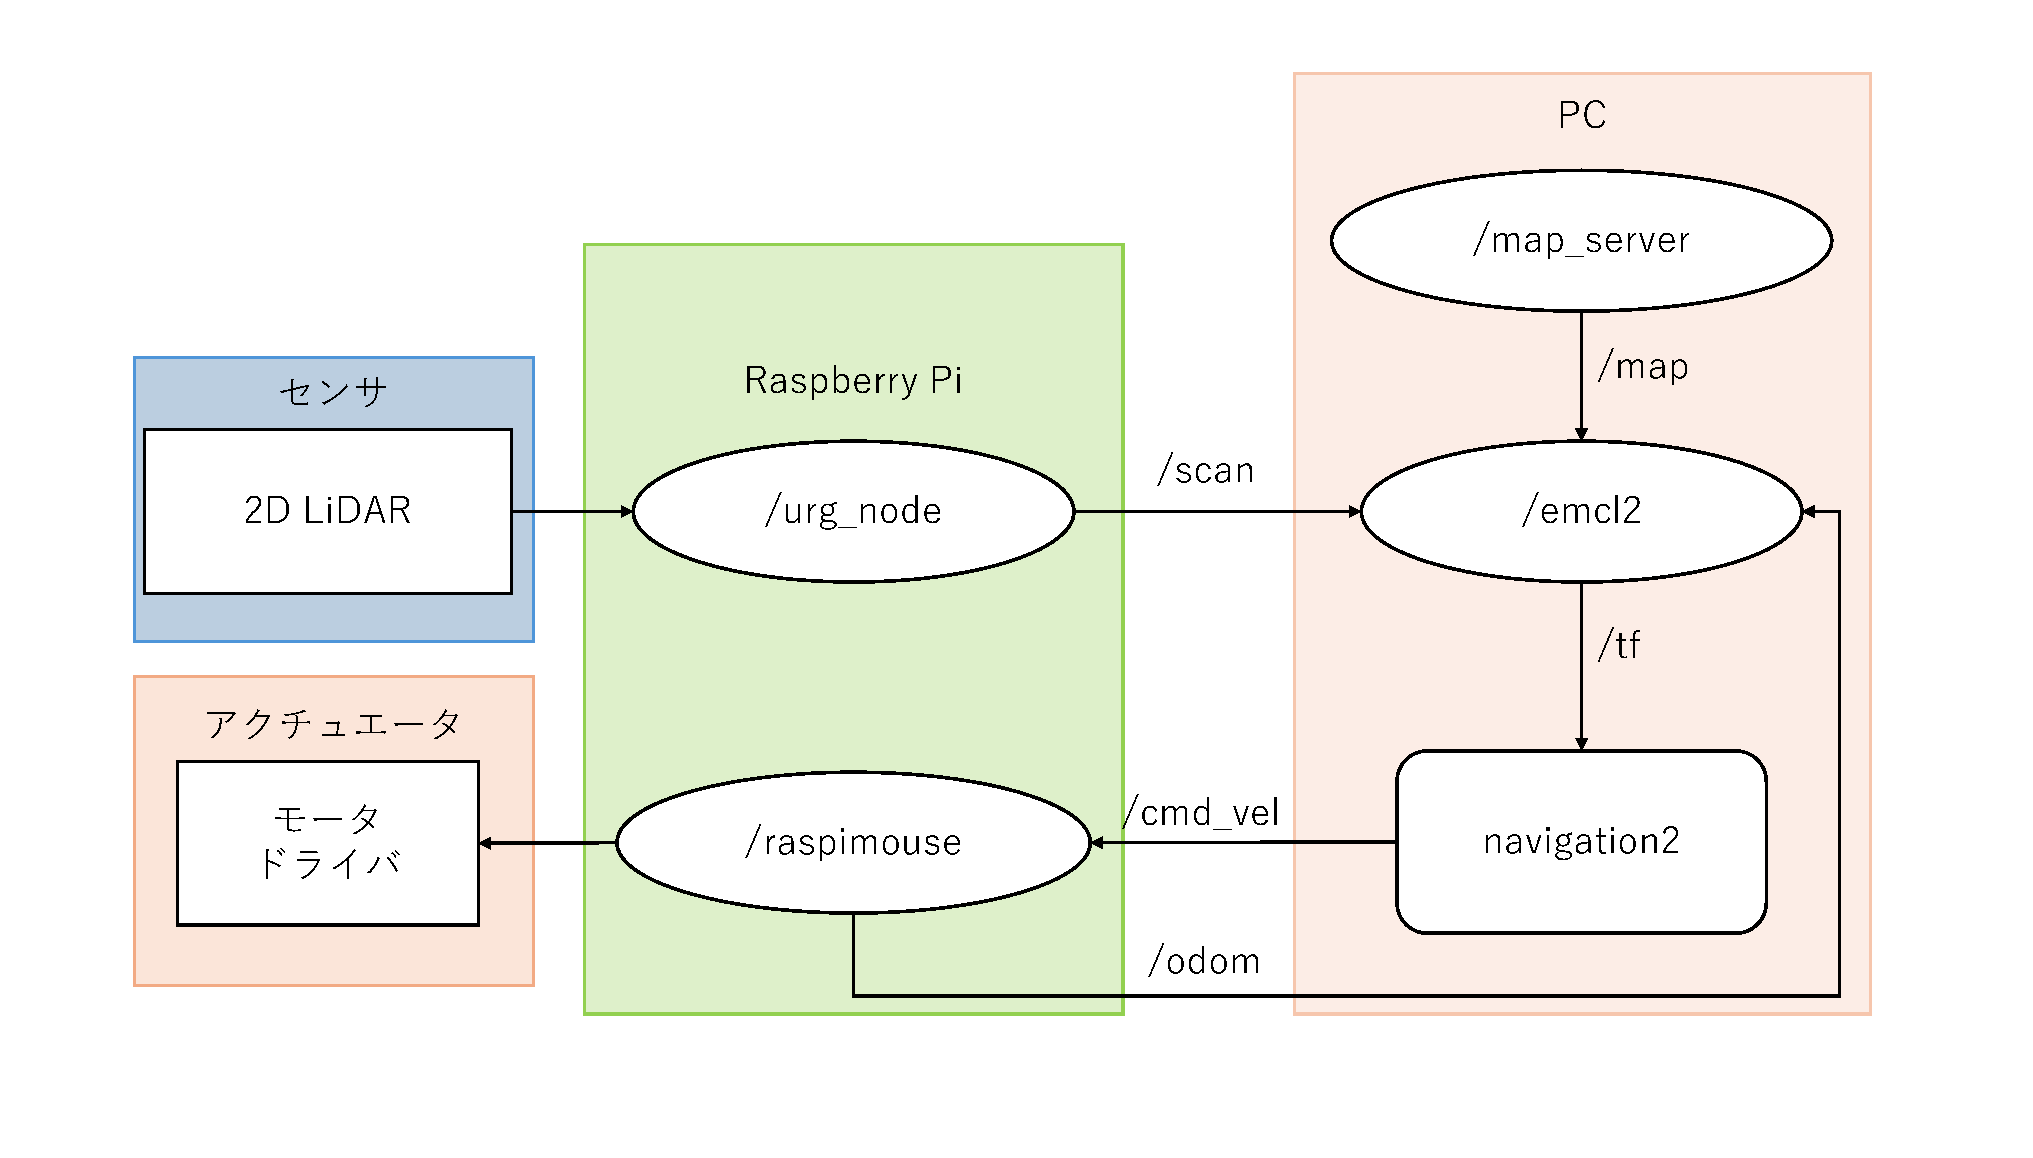
\includegraphics[width=1.0\linewidth]{figs/shiratama_system_diagram.eps}
    \caption{しらたまチームのシステム構成}
    \label{fig:shiratama_system}
  \end{center}
\end{figure}
